\documentclass[12pt]{article}
\usepackage{amsmath, slashed, fullpage,hyperref}
	\usepackage{graphicx, bbold}
	\usepackage{verbatim, booktabs}
	\usepackage{animate, listings}
	\usepackage{xcolor, tcolorbox}
	\usepackage[final]{pdfpages}
	
	
	\definecolor{commentsColor}{rgb}{0.24, 0.24, 0.24}
	\definecolor{keywordsColor}{rgb}{1.0, 0.4, 0.4}
	\definecolor{stringColor}{rgb}{0.125, 0.067, 0.949}
	
	\lstset{ %
		backgroundcolor=\color{white},   % choose the background color; you must add \usepackage{color} or \usepackage{xcolor}
		basicstyle=\footnotesize,        % the size of the fonts that are used for the code
		breakatwhitespace=false,         % sets if automatic breaks should only happen at whitespace
		breaklines=true,                 % sets automatic line breaking
		captionpos=b,                    % sets the caption-position to bottom
		commentstyle=\color{commentsColor}\textit,    % comment style
		deletekeywords={...},            % if you want to delete keywords from the given language
		escapeinside={\%*}{*)},          % if you want to add LaTeX within your code
		extendedchars=true,              % lets you use non-ASCII characters; for 8-bits encodings only, does not work with UTF-8
		frame=tb,	                   	   % adds a frame around the code
		keepspaces=true,                 % keeps spaces in text, useful for keeping indentation of code (possibly needs columns=flexible)
		keywordstyle=\color{keywordsColor}\bfseries,       % keyword style
		language=Go,                 % the language of the code (can be overrided per snippet)
		otherkeywords={*,...},           % if you want to add more keywords to the set
		numbers=left,                    % where to put the line-numbers; possible values are (none, left, right)
		numbersep=5pt,                   % how far the line-numbers are from the code
		numberstyle=\tiny\color{commentsColor}, % the style that is used for the line-numbers
		rulecolor=\color{black},         % if not set, the frame-color may be changed on line-breaks within not-black text (e.g. comments (green here))
		showspaces=false,                % show spaces everywhere adding particular underscores; it overrides 'showstringspaces'
		showstringspaces=false,          % underline spaces within strings only
		showtabs=false,                  % show tabs within strings adding particular underscores
		stepnumber=1,                    % the step between two line-numbers. If it's 1, each line will be numbered
		stringstyle=\color{stringColor}, % string literal style
		tabsize=4,	                   % sets default tabsize to 2 spaces
%		title=\lstname,                  % show the filename of files included with \lstinputlisting; also try caption instead of title
		columns=fixed                    % Using fixed column width (for e.g. nice alignment)
	}


\usepackage{hyperref, fullpage, amsmath, amsthm, amssymb, graphicx, tikz}
\hypersetup{colorlinks=true, linkcolor=blue, filecolor=blue, urlcolor=blue, citecolor=blue}
\newenvironment{question}{\noindent\underline{\textbf{Question}}:\quad}{\\}
\newenvironment{solution}{\noindent\underline{\textbf{Solution}}:\quad}{\\}

\begin{document}
	\hspace*{-0.6cm}
	\begin{minipage}{0.5\linewidth}
		\underline{\textbf{Name}}:\quad Bryce Chudomelka\\
		\underline{\textbf{Class}}:\quad COMP605
	\end{minipage}
	\hfill
	\begin{minipage}{0.24\linewidth}
		\underline{\textbf{RedID}}:\quad 823380825\\
		\underline{\textbf{Date}}:\quad \today
	\end{minipage}\\
	\noindent\rule{\textwidth}{0.25pt}
	\section*{Final Project}
		The current state of High Performance Computing (HPC) is done in ancient languages such as C/C++ or Fortran. These languages are extremely low-level, \textit{i.e.} the computer language is closer to the machine code than a high-level language like Python, which makes them efficient for computation. The drawback is that these languages were designed at a time when only one core processors were in production. Today's computing environments utilizes central processing units (CPUs) with many cores and each core having two threads, thus allowing many operations to be performed concurrently. We can benchmark the potential performance increase on a matrix-matrix multiplication algorithm, see Figure \ref{fig:ABC}.\\
		
		Concurrency is the most likely the principal design of the computing language Go, aka ``Concurrency made easy by Google." Developed in 2009 by Google, Go is a language that borrows from C/C++ but is designed with multi-core CPUs in mind. With regards to HPC, concurrency can be done in C/C++ using a variety of techniques such as \texttt{pthreads}, \texttt{OpenMP}, or \texttt{MPI}, which are not native to the language itself, and impose restrictions in development by requiring complex code. Many of these concerns have been addressed in the development of Go and are native to the language itself without syntactic sugar.
		
	
		\subsection*{Concurrency made easy}
			Go's syntax for performing concurrency is as simple as typing \texttt{go }. In just three characters, \texttt{g}, \texttt{o}, and a space, a light-weight operation, known as a \texttt{goroutine}, is spawned. A \texttt{goroutine} is similar to a thread that is created by \texttt{pthreads}, but is handled by the \texttt{Go} runtime without additional code complexity. The \texttt{Go} runtime identifies the number of CPUs available and sets a variable known as \texttt{GOMAXPROCS} to optimize the number of \texttt{goroutines} that can be concurrently spawned.\\
			
			\begin{figure}[b]
				\centering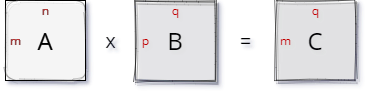
\includegraphics[width=0.618\textwidth]{../imgs/ABC}
				\caption{Matrix-matrix multiplication of two non-square matrices $A_{m\times n}\times B_{p\times q}$ yields a matrix $C_{m\times q}$; assuming $n=p$. This problem has $\mathcal{O}(mnp)$ time complexity naively, which can be reduced in a myriad of ways..}
				\label{fig:ABC}
			\end{figure}
			
			In HPC we utilize threads to perform tasks concurrently to optimize computation. We have already observed in class that the time complexity of a given program can be drastically reduced by performing concurrent operations. Also, we observed that using more threads does not always directly lead to performance increases. This is easily observed when trying to spawn more threads than 2 times the number of CPUs, roughly speaking. This introduces a possible bottleneck for computation though with current hardware restrictions; current CPUs have 8-32 cores, at most.
			
		\subsection*{Distributed computing} 
			We can access more threads if we add more CPUs, but this problem requires us to add another machine. \texttt{MPI} is a message passing interface implemented in \texttt{C} that allows the use of many machines for distributed computation. Thus, giving the user access to more CPUs, \textit{i.e.}, threads, to improve computation and reduce time complexity. As shown in a previous homework, I found an MPI-like package in \texttt{Go} and implemented it successfully to test the network bandwidth, \textit{e.g.}, determining the latency of sending bytes across ports on the same machine. While that exercise was useful, the more challenging problem is communicating across machines in the network.\\
			\begin{figure}
				\centering
\includegraphics[width=0.618\textwidth]{../imgs/clientserver1}
				\caption{Half of the computation is split between the client and the server. Both machines receive an equal amount of work.}
				\label{fig:cs1}
			\end{figure}
		
			We can simulate this behavior using a TCP connection between two machines to pass information; see Figure \ref{fig:cs1}. Bytes of information can be sent across the network for a relatively low cost, \textit{e.g.}, latency as seen in a recent homework, but memory cannot be shared across a TCP connection. This adds an additional operation of combining the distributed computation into its final form. Some might call it, "the cost of doing business," because adding \textit{unneeded} operations to the task should increase run time. This will be addressed in the analysis section.
		
		\subsection*{Methodology}
			\begin{figure}
				\centering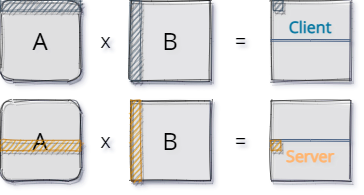
\includegraphics[width=0.618\textwidth]{../imgs/clientserver2}
				\caption{This visualization shows how either the client or the server perform their piece of the computation. This allows us to easily combine the resultant matrix after computation.}
				\label{fig:cs2}
			\end{figure}
			In this project, a proof-of-concept has been created to distribute computational resources across two machines. I will connect two nodes on the server \texttt{tuckoo.sdsu.edu} via a transmission control protocol (TCP) connection, where the instructions will be sent in a client/server paradigm to distribute computation between two machines. The client will be responsible for initializing and populating the matrices, as, providing the server with instructions, combining the results, as well as doing half the work in matrix-matrix multiplication. The server will listen and wait until it receives a message from the client then perform the matrix-matrix multiplication as indicated and return the results via TCP.\\

			Matrix-matrix computation is costly when performed in serial, and we will utilize the \texttt{goroutine} version created in a previous homework assignment to improve performance when compared to the traditional row-wise multiplication algorithm. Only a slight modification needs to be made to indicate starting row and ending row for computation. Each machine will perform their portion of matrix-matrix computation using \texttt{goroutines}, thus effectively turning a big problem for one machine into a smaller problem for two machines; see Figure \ref{fig:cs2}. We note that for small matrices this is sub-optimal due to network latency and the added operation of combining two matrices.\\

			First, the client will initialize three slices of floats according to the input parameters. Next, the client will determine which rows of the matrix $C$ that the both the client and server has to compute, then pass the required information via a \texttt{struct} to the server. At this point in the client/server paradigm, each machine begins to perform their individual tasks according to the \texttt{goRowMultMat} function, which performs row-wise matrix multiplication on a flattened matrices using \texttt{goroutines}. After the server finishes its work, the server then dials up the client via TCP and sends over its half of the resultant matrix along with the number of \texttt{goroutines} used. Finally, the client combines the two results and exits the program. Even though the algorithm is designed to multiply non-square matrices, the benchmarks performed in this experiment will only consider square matrices, \textit{i.e.} $A_{n\times n}\times B_{n\times n}=C_{n\times n}$, to simplify analysis.
			
		\subsection*{Results}
			We perform matrix-matrix multiplication on \texttt{tuckoo.sdsu.edu}, a network of CPUs with various properties. We will multiply matrices where $n$ will take on various values. The results of the experiments are tabulated in Table \ref{tab:results}. The computation time will be measured, in seconds, for each run as well.
			
			\begin{table}
				\centering
				\begin{tabular}{|c||c|c|c|}
					\hline
					  $n$&     Row  &Goroutine&Distributed\\\hline\hline
					  250&    0.049 &   0.007 &  0.022\\\hline
					  500&    0.395 &   0.034 &  0.072\\\hline
					  750&    1.354 &   0.105 &  0.164\\\hline
					 1000&    2.920 &   0.217 &  0.300\\\hline
					 1250&    6.118 &   0.435 &  0.501\\\hline
					 1500&   10.103 &   0.723 &   0.786\\\hline
					 1750&   34.168 &   2.177 &   1.439\\\hline
					 2000&   41.578 &   2.874 &   1.902\\\hline
					 2250&   77.667 &   4.555 &   3.137\\\hline
					 2500&   93.060 &   5.463 &   3.694\\\hline
					 5000&  820.133 &  43.913 &  25.819\\\hline
					 7500& 3573.429 & 175.860 &  95.659\\\hline
					10000& 6558.381 & 353.265 & 203.442\\\hline
					15000&     *    &1318.689 & 702.739\\\hline
					20000&     *    &9400.968 & 3656.001\\\hline
				\end{tabular}
				\caption{The results of each trial run are compiled here with each timing being measured in seconds. Here Row refers to row-wise, Goroutines to single-machine, and Distributed to matrix-matrix multiplication; respectively.}
				\label{tab:results}
			\end{table}
		
			\begin{figure}
				\centering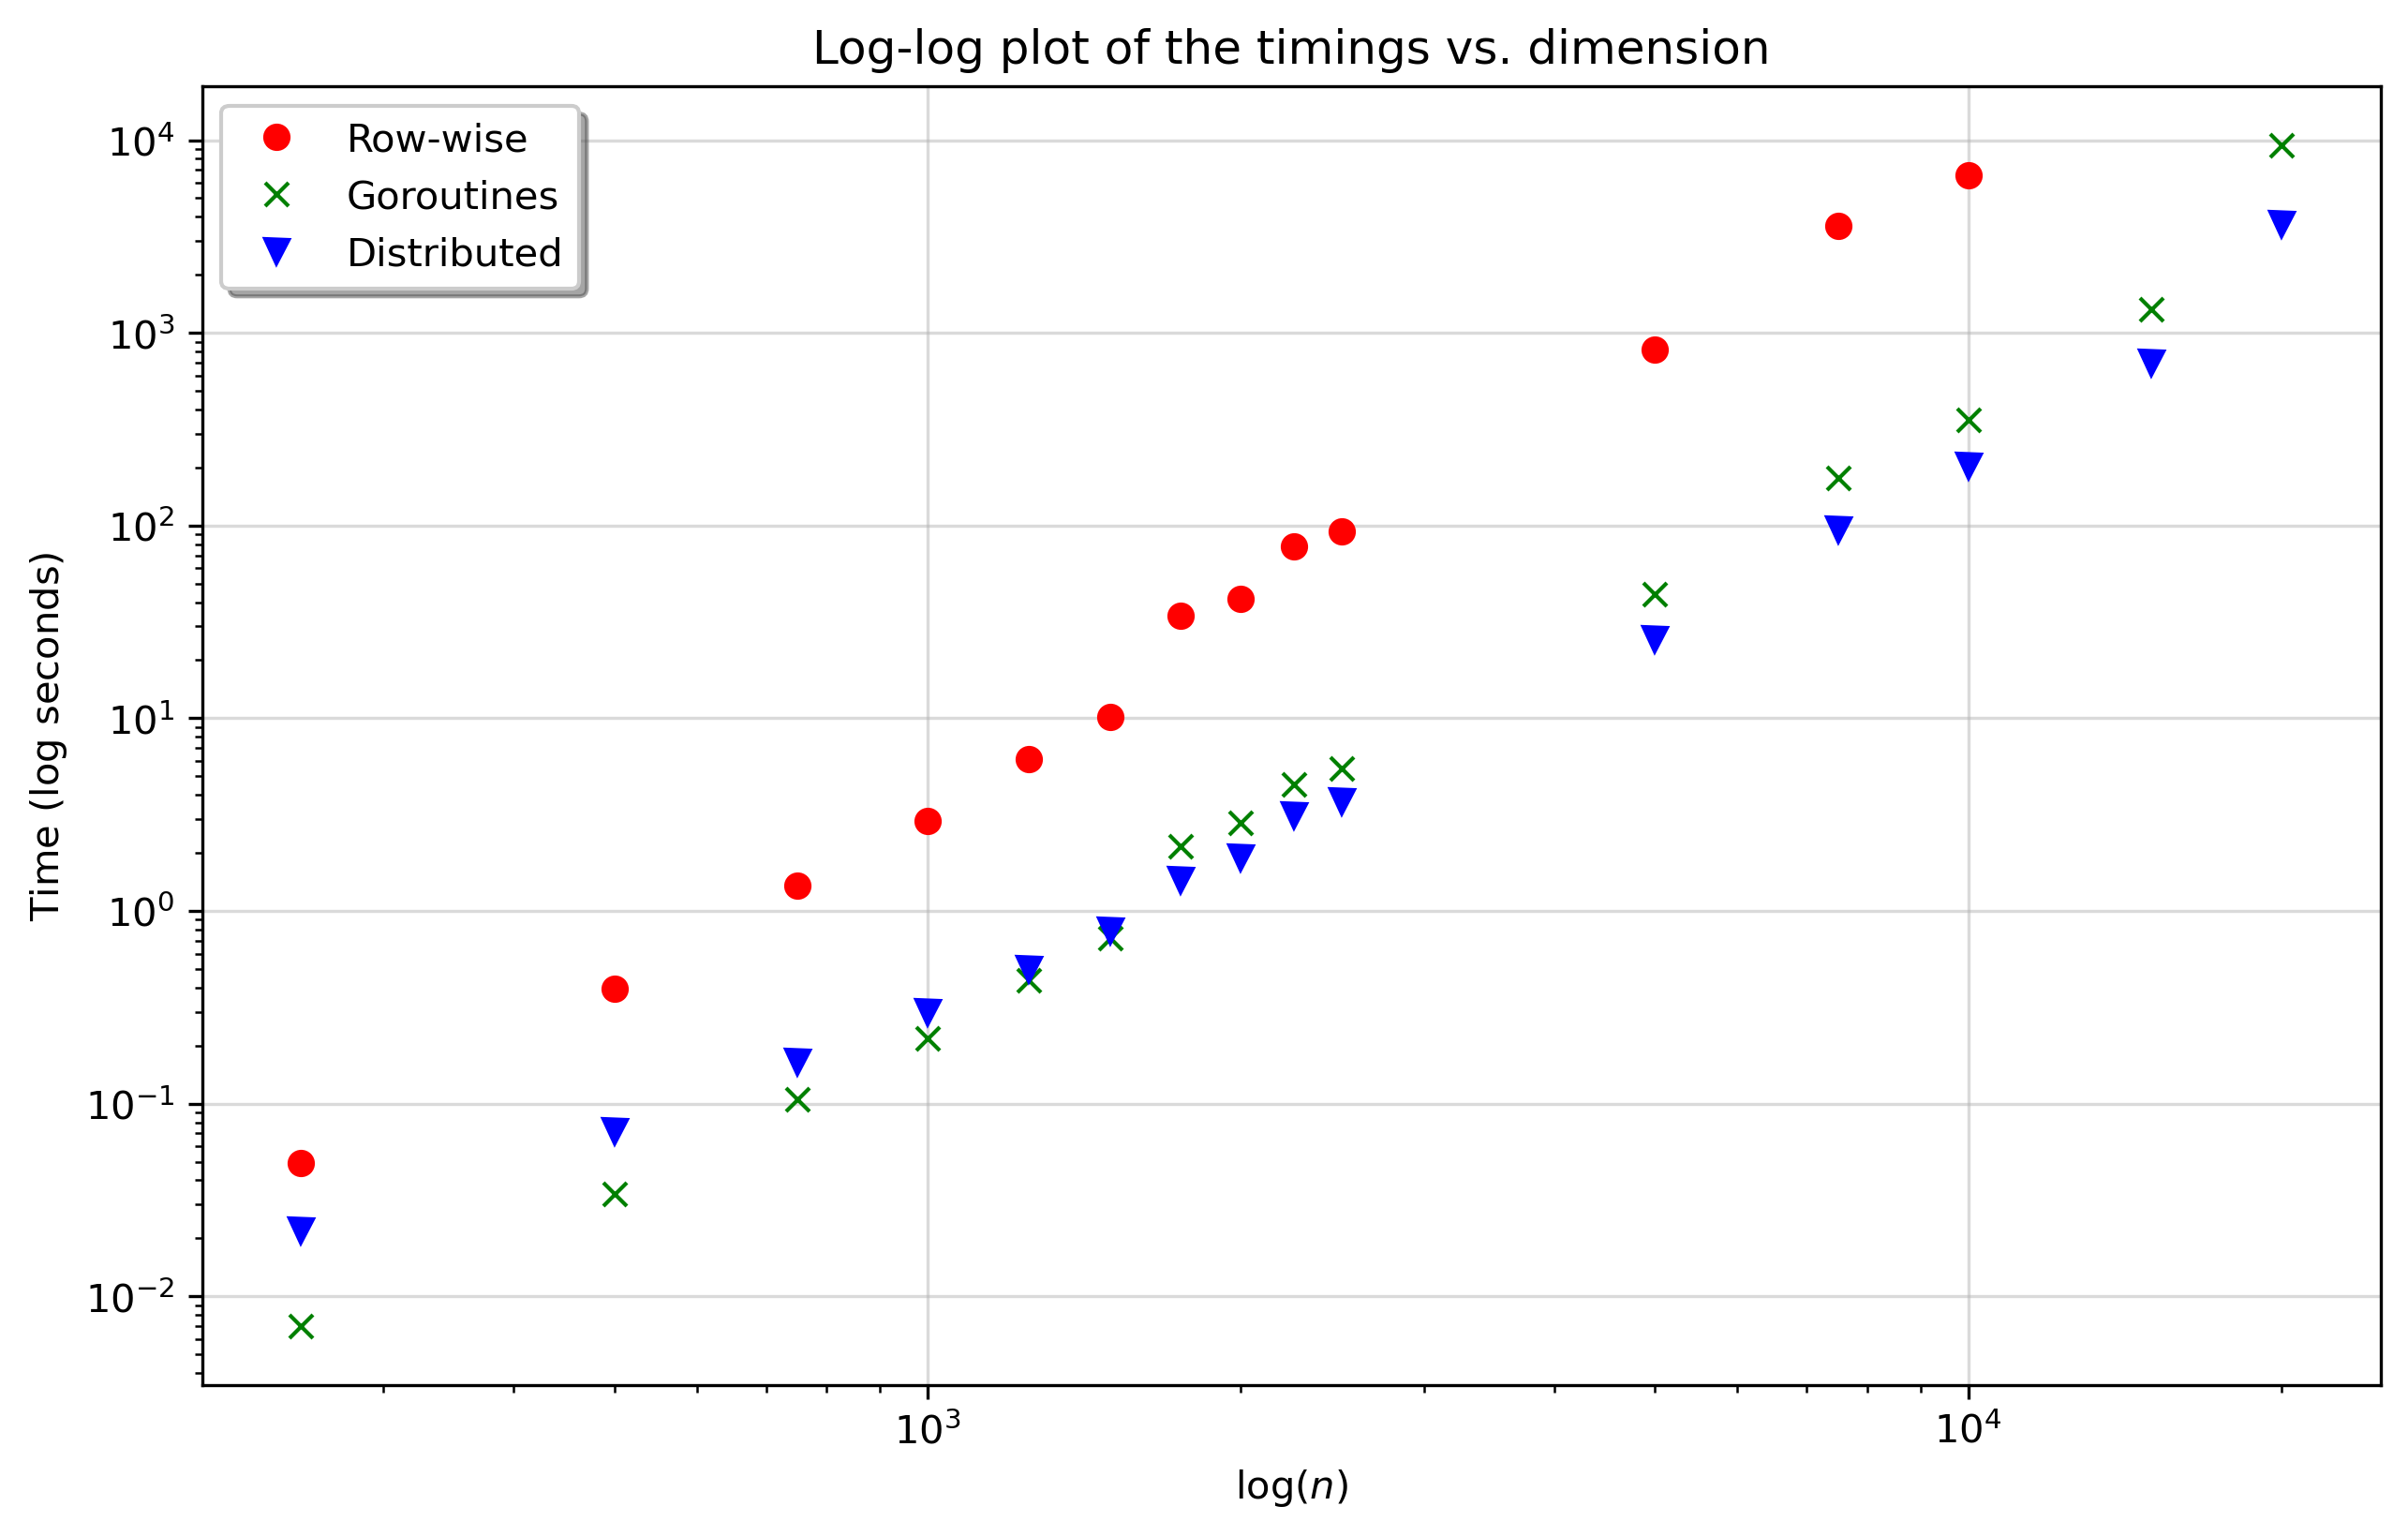
\includegraphics[width=0.7618\textwidth]{../imgs/results}
				\caption{This visualization shows how either the client or the server perform their piece of the computation. This allows us to easily combine the resultant matrix after computation.}
				\label{fig:results}
			\end{figure}
		
		\subsection*{Analysis}					
			The time complexity associated with row-wise matrix-matrix multiplication is observed to be significantly worse than the Goroutine algorithm. It is important to distinguish between the Goroutine algorithm and the distributed method. It was measured that the Goroutine method used 16 threads and that the distributed method between \texttt{node10} and \texttt{node12} was 32. There is a cost associated with sending the data across the network and combining the received results.\\
			
			As $n$ increases, the cost associated with distributing the computation diminishes to the point where distributed computation out performs goroutines. This is reflective of the number of threads/goroutines and how there is a performance bottleneck. A simple threaded algorithm on one machine is sufficient to perform matrix-matrix multiplication until the size of the matrices surpasses a particular amount, which we observe to be roughly $n=2000$. Distributed computation is more performant than single machine threaded, or serial, computation whenever the dimension of the matrices are too large.\\
			
		\subsubsection*{Drawbacks}
			Sometimes we view the world through rose-colored glasses and it can simply be put as, ``Not all problems are alike!" This is correct because depending on the parameters of your problem, \textit{i.e.}, dimension size, one should be careful about the algorithm/methodology used to solve their problem. If you are trying to solve a 3$\times$3 matrix, then a trivial row-wise matrix-matrix multiplication would ``make-sense". The problem is that when we try to scale up our input dimensions that our algorithms become slow, less performant, and inefficient. Thus, we must introduce distributed computing, in order to accommodate for increased input dimensions once our matrix size is sufficiently large. Scientific computing at scale \textit{requires} distributed computing. This experiment loosely demonstrates that as a proof-of-concept. A final note that more care should be taken when computing timings to consider the average with some tolerance for a true benchmark.
			
		\subsubsection*{Future Work}
			\begin{figure}
				\centering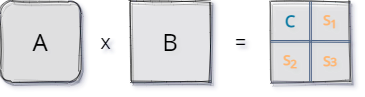
\includegraphics[width=0.618\textwidth]{../imgs/clientserver3}
				\caption{This visualization shows how either the client or server perform their piece of the computation; an example using 4 nodes labeled $C, S_1, S_2,$ and $S_3$ is depicted here where $C$ is the client, and $S_1,S_2,S_3$ are the server nodes. This allows us to easily combine the resultant matrix after computation.}
				\label{fig:cs3}
			\end{figure}
			This work can now easily be extended to include more machines in a network. If the number of nodes being used is odd then divvy up the rows in the output matrix C accordingly, but if the number of nodes is even, and greater than 2, then split on the columns, as seen in Figure \ref{fig:cs3}. This pattern can alternate rows and columns as needed. Care should be taken on behalf of the client side as to receive all results before combining, but that is a problem for another day.
			
	\newpage
	\subsection*{Code}
		\subsubsection*{Row}
			\lstinputlisting{../matmul.go}
		\subsubsection*{Client}
			\lstinputlisting{../client.go}
		\subsubsection*{Server}
			\lstinputlisting{../server.go}
		\subsubsection*{Results}
			\lstinputlisting[language=Python]{../results.py}
			
			
\end{document}
